\section{Implementation and results} \label{sec:results}
This project implemented the different approaches to selective identification of IP devices proposed in \cref{sec:method}. These implementations, along with a discussion of the results, will be described here. 


\subsection{Banner similarities} \label{sec:banner_results}
Following the approach proposed in \cref{sec:banner_method}, the first step is to choose a type of device that could fit the constraints of this project. Two methods was used to find a such a device. The first one was to find other research into the same area, and look at their results. Google Scholar\cite{google_scholar} and Engineering Village\cite{engineering_village} was used in search for articles on the subject, while DuckDuckGo\cite{ddg} was used to search for other sources. A powerpoint presentation from the Hack In The Box Security Conference 2018 was found, named \textit{Hacking yachts remotely}. This presentation illustrates different methods to hack Yachts. Here the search query "Maritime Sabolized Antenna System" was used to find internet connected antennaes of the model "Cobham Seatel Satcom". 
"Marine Stabilized Antenna System" would then be an identifying part of the banner of this device. The 22 results found when using Shodan to search for this can be found in \cref{fig:banner_parsing}. Note that all devices run on the same port: 161, which is used for the Simple Network Management Protocol (SNMP). This will be looked further into in \cref{sec:combo}.

\begin{figure} [H]
    \centering
    \includegraphics[scale=0.4]{Figurer/banner_parsing.png}
    \caption{Using the Shodan CLI to download and parse results. Results are listed with IP addresses, open ports and ISP.}
    \label{fig:banner_parsing}
\end{figure}

In the millions of devices connected to the internet, 22 devices is not really very many. However, this is the most accurate device identification this project was able to do. While the other approaches are also able to identify devices, it is not ceritan that those are a part of the offshore or maritime industries. The Cobham Seatel Satcom antenna is definetly a part of the navigation system of a ship, which is a maritime Cyber-Physical System. This one result was also one not found by this project, but by another project. More specifically, it was found by someone who has more insight into the industry, showing that device identification by banner specification is easier with experience from area of work within the constraints or access to relevant devices.

If this experience or access is not available, like in this project, a couple of methods can be used to search for identifying device banners. 
Some techonologies are intended for specialized use. For example the NMEA communication standard for marine sensors and display units. \cite{NMEA} This will of course be mostly used in the marine industry. A shodan search for "NMEA" shows that 88 IP addresses have the word NMEA in their description. While some of those devices probably use NMEA to communicate, some might just have the letters "NMEA" in their banner as a coincidence. This can be the case with short search terms. The port 10110 is intended for NMEA 0183 Navigational Data. \cite{www_ports} A search for this port with Shodan returns 6 results, which is quite low. 
It is possible to find devices that are used within a industry, in this case either maritime or offshore. These devices need to be specific for the industry, as findings will not be decisive if the devices can be found in used not within the constraints. To find the right devices, one approach can be to find producers or resellers of equipment for a specific industry. A list of manufacturers of NMEA equipment can be found at \cite{NMEA}. It is logical that some of these manufacturers would also make equipment for the marine industry that is not NMEA. 
This project spent some time \todo[inline]{Finish this section by adding results from table or smoething.}


\subsection{ISP}
For identifying devices by looking at Internet Service Providers (ISP), Tampnet will be used as an example. On their webpage, the follwing can be found: "By providing a fast subsea fibre optic network and 4G LTE coverage, Tampnet enables digitalization of offshore operations within oil \& gas, maritime and wind energy." \cite{tampnet} Tampnet is an ISP that provides internet connections to the maritime, offshore and wind energy industries. 

\begin{figure} [H]
    \centering
    \includegraphics[scale=0.35]{Figurer/python_ports.png}
    \caption{The output from a python script that is counting the different number of ports open by the devices returned from the Shodan query "isp:tampnet". The script is "count\_ports.py" at \cite{scripts}}
    \label{fig:tampnet_ports}
\end{figure}

This query returns 92 different IP addresses belonging to Tampnet. This approach is not definitive, however, since there is no way of knowing if these devices are a part of a cyber-physical system in the offshore industry. Even so, these 92 devices has a higher chance of being within the constraints than other random devices on the internet. This method will thus act more as a filter for finding potential hits. 

The HackerTargets AS lookup tool \cite{asip_lookup} is used to find that Tampnet own the CIDR range "185.96.40.0/22", which is 1024 available IP addresses. \cite{CIDR_table} Therefore, Tampnet probably has more than 92 active IP addresses as part of their ISP. Shodan can not find the rest of the IP addresses of Tampnet since they can not be reached from the public internet. One reason for this could be that Tampnet employs a firewall to filter what IP addresses are able to find their address. This is called whitelisting, where only a selected number of devices can communicate through the router with a firewall, as illustrated in \cref{fig:firewall}.


\tikzset{every picture/.style={line width=0.75pt}} %set default line width to 0.75pt
\begin{tabular}{p{10cm}}
    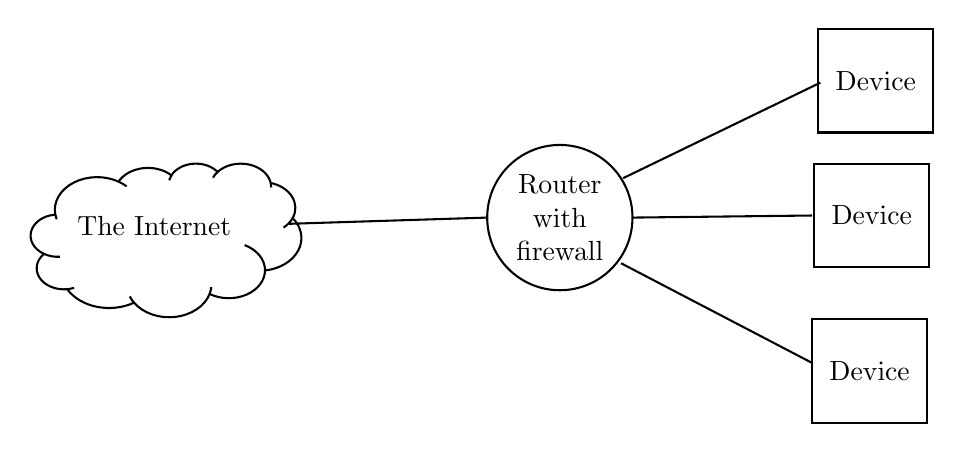
\begin{tikzpicture}[x=0.75pt,y=0.75pt,yscale=-1,xscale=1]
        %uncomment if require: \path (0,300); %set diagram left start at 0, and has height of 300

        %Shape: Rectangle [id:dp7550808737565868]
        \draw   (417.5,74) -- (473,74) -- (473,124) -- (417.5,124) -- cycle ;

        %Shape: Ellipse [id:dp5744265006375734]
        \draw   (258,165) .. controls (258,145.67) and (273.67,130) .. (293,130) .. controls (312.33,130) and (328,145.67) .. (328,165) .. controls (328,184.33) and (312.33,200) .. (293,200) .. controls (273.67,200) and (258,184.33) .. (258,165) -- cycle ;

        %Straight Lines [id:da011152119100300673]
        \draw    (418.5,100) -- (323.5,146) ;
        %Shape: Rectangle [id:dp019726233695570805]
        \draw   (414.5,214) -- (470,214) -- (470,264) -- (414.5,264) -- cycle ;

        %Shape: Rectangle [id:dp2854982925574172]
        \draw   (415.5,139) -- (471,139) -- (471,189) -- (415.5,189) -- cycle ;

        %Straight Lines [id:da042657718924057675]
        \draw    (414.5,164) -- (328,165) ;
        %Straight Lines [id:da8590380439733557]
        \draw    (414.5,235) -- (322.5,187) ;
        %Shape: Cloud [id:dp5209862047408297]
        \draw   (49.88,163.36) .. controls (48.82,157.4) and (52.27,151.49) .. (58.76,148.15) .. controls (65.25,144.81) and (73.64,144.62) .. (80.36,147.67) .. controls (82.74,144.2) and (87.1,141.8) .. (92.13,141.21) .. controls (97.15,140.61) and (102.24,141.88) .. (105.86,144.64) .. controls (107.89,141.49) and (111.87,139.38) .. (116.4,139.05) .. controls (120.93,138.71) and (125.35,140.21) .. (128.11,143.01) .. controls (131.78,139.67) and (137.61,138.27) .. (143.09,139.4) .. controls (148.57,140.54) and (152.7,144) .. (153.71,148.31) .. controls (158.2,149.25) and (161.95,151.66) .. (163.97,154.91) .. controls (166,158.15) and (166.1,161.92) .. (164.27,165.23) .. controls (168.7,169.68) and (169.73,175.61) .. (166.99,180.8) .. controls (164.25,186) and (158.14,189.68) .. (150.95,190.48) .. controls (150.9,195.35) and (147.44,199.83) .. (141.9,202.17) .. controls (136.37,204.52) and (129.62,204.38) .. (124.26,201.79) .. controls (121.98,207.63) and (115.55,211.93) .. (107.76,212.83) .. controls (99.97,213.73) and (92.21,211.06) .. (87.83,205.99) .. controls (82.46,208.49) and (76.02,209.21) .. (69.96,207.99) .. controls (63.9,206.77) and (58.74,203.7) .. (55.62,199.49) .. controls (50.14,199.99) and (44.84,197.79) .. (42.35,194) .. controls (39.86,190.2) and (40.71,185.61) .. (44.49,182.5) .. controls (39.59,180.28) and (37.1,175.87) .. (38.3,171.56) .. controls (39.5,167.26) and (44.13,164.05) .. (49.76,163.59) ; \draw   (44.49,182.5) .. controls (46.8,183.55) and (49.46,184.03) .. (52.13,183.87)(55.62,199.49) .. controls (56.77,199.39) and (57.89,199.17) .. (58.97,198.84)(87.83,205.99) .. controls (87.02,205.06) and (86.34,204.06) .. (85.81,203.01)(124.26,201.79) .. controls (124.67,200.73) and (124.95,199.63) .. (125.06,198.52)(150.95,190.48) .. controls (151.01,185.28) and (147.19,180.53) .. (141.14,178.26)(164.27,165.23) .. controls (163.29,167) and (161.79,168.57) .. (159.9,169.81)(153.71,148.31) .. controls (153.88,149.02) and (153.95,149.75) .. (153.94,150.47)(128.11,143.01) .. controls (127.2,143.84) and (126.44,144.77) .. (125.87,145.77)(105.86,144.64) .. controls (105.37,145.39) and (105.01,146.19) .. (104.77,147.02)(80.36,147.67) .. controls (81.78,148.31) and (83.1,149.09) .. (84.28,149.97)(49.88,163.36) .. controls (50.02,164.19) and (50.25,165) .. (50.56,165.79) ;

        %Straight Lines [id:da9624009852798121]
        \draw    (162.5,168) -- (258,165) ;

        % Text Node
        \draw (293,165) node   [align=left] {\begin{minipage}[lt]{33.354pt}\setlength\topsep{0pt}
            \begin{center}
                Router\\ with \ firewall
            \end{center}

        \end{minipage}};
        % Text Node
        \draw (445.25,99) node   [align=left] {Device};
        % Text Node
        \draw (442.25,239) node   [align=left] {Device};
        % Text Node
        \draw (443.25,164) node   [align=left] {Device};
        % Text Node
        \draw (59,163) node [anchor=north west][inner sep=0.75pt]   [align=left] {The Internet};

    \end{tikzpicture}
    \captionof{figure}{Illustration of firewall functionality}
    \label{fig:firewall}
\end{tabular}




\subsection{Reverse Geolocation}
With many major seaports, like Rotterdam, Antwerp and Hamburg, the North Sea has a lot of marine traffic. The sea also has a lot of offshore oil and gas fields; Ekofisk, Sleipner, Forties and Valhall, to mention a few.\cite{oil_field_lists} With this much activity within both constraints, the marine and offshore industries, a lot of things in the area have to be connected to the internet. To test if the IP geolocation services of Shodan could detect devices connected to the internet, a large area of the North sea was chosen: a circle with 270 km around 56\degree24\textquotesingle00.0N 3\degree00\textquotesingle36.0E, as seen in \cref{fig:geolocation}. To use Shodan to find devices within this area, the command \cref{lst:geolocation_sea} was used. As seen in the output from the command, no devices was found within the area. The command syntax is "shodan count geo:LONGITUDE,LATITUDE,RADIUS"

\begin{figure} [H]
    \centering
    \includegraphics[scale=0.7]{Figurer/geolocation.png}
    \caption{Shodan "geo" filter visualized. Map copyright: https://www.openstreetmap.org/copyright}
    \label{fig:geolocation}
\end{figure}

This query returns zero hits, which shows that the reverse geolocation approach does not work. One possible explanation for this is that the devices are registered in one location, while they are physically located at another. As mentioned in \cref{sec:geo_method}, it is not clear how shodan find locations, and therefore hard to decide how accurate te information can be.

\subsection{Latency and traceroute}
As this project does not have access to any tools that index traceroute latencies, it is not possible to parse trough large quentities of IP address latencies. Therefore, to show how this approach works, the Cobham Seatel Satcom antenna example from \cref{sec:banner_results} will be used, as these devices is already confimed within the constraints. The traceroute command is simple: "traceroute IP\_ADDRESS". A graph of the latencies from the traceroute can be seen in \cref{fig:traceroute_graph}.

\begin{figure} [H]
    \centering
    \includegraphics[scale=0.7]{Figurer/latency_graph_marked.png}
    \caption{A visualization of the mean latencies from the traceroute command on the IP address 216.236.193.173.}
    \label{fig:traceroute_graph}
\end{figure}

Two points on this graph is worth mentioning. The first point (1), where the latency has a \~200ms jump, could be a undersea cable.From a Shodan query for the destination IP address, it is found to be in USA, so this is probably when the signal crosses the Atlantic Ocean. The next point on the graph (2), increase the latency by \~1000ms. As the antenna is connected to the internet via sattelite, this is probably when the signal travel from land, trough the sattelite to the antenna.

With access to large datasets of traceroute latencies, it could be possible to identify devices that have big latency jumps. While this could not prove that a device is located at sea, it would be useful to find subsets of IP addresses that could be investigated further.

\subsection{Comparison of methods}
The different methods discussed in this section show different strengths and weaknesses. Here the main things to remember from each are shown in a list.

\begin{outline}[itemize]
        \1 Banner Similarities
            \2 Pinpoint an exact device model
            \2 Hard to find identifying device banner
        \1 Internet Service Provider and IP ranges
            \2 Will give a subset of devices possibly within constraints
        \1 Reverse IP geolocation
            \2 Does not work
        \1 Latency and traceroute
            \2 Can be used to give more confidence in identyfing a device.
\end{outline}

\subsection{Combination of methods} \label{sec:combo}
\todo[inline]{Maybe write this chapter}

\subsection{ICS}
\todo[inline]{Maybe write this chapter}

\subsection{ECDIS}
\todo[inline]{Maybe write this chapter}
